%%%%%%%%%%%%%%%%%%%%%%%%%%%%%%%%%%%%%%%%%%%%%%%%%%%
%% LaTeX book template                           %%
%% Author:  Amber Jain (http://amberj.devio.us/) %%
%% License: ISC license                          %%
%%%%%%%%%%%%%%%%%%%%%%%%%%%%%%%%%%%%%%%%%%%%%%%%%%%

\documentclass[a4paper,11pt,oneside]{book}
\usepackage{../../modulestyle}

%%%%%%%%%%%%%%%%%%%%%%%%%%%%%%%%%%%%%%%%%%%%%%%%%%%%%%%%%
% Source: http://en.wikibooks.org/wiki/LaTeX/Hyperlinks %
%%%%%%%%%%%%%%%%%%%%%%%%%%%%%%%%%%%%%%%%%%%%%%%%%%%%%%%%%

%%%%%%%%%%%%%%%%%%%%%%%%%%%%%%%%%%%%%%%%%%%%%%%%%%%%%%%%%%%%%%%%%%%%%%%%%%%%%%%%
% 'dedication' environment: To add a dedication paragraph at the start of book %
% Source: http://www.tug.org/pipermail/texhax/2010-June/015184.html            %
%%%%%%%%%%%%%%%%%%%%%%%%%%%%%%%%%%%%%%%%%%%%%%%%%%%%%%%%%%%%%%%%%%%%%%%%%%%%%%%%
\newenvironment{dedication}
{
   \cleardoublepage
   \thispagestyle{empty}
   \vspace*{\stretch{1}}
   \hfill\begin{minipage}[t]{0.66\textwidth}
   \raggedright
}
{
   \end{minipage}
   \vspace*{\stretch{3}}
   \clearpage
}

%%%%%%%%%%%%%%%%%%%%%%%%%%%%%%%%%%%%%%%%%%%%%%%%
% Chapter quote at the start of chapter        %
% Source: http://tex.stackexchange.com/a/53380 %
%%%%%%%%%%%%%%%%%%%%%%%%%%%%%%%%%%%%%%%%%%%%%%%%
\makeatletter
\renewcommand{\@chapapp}{}% Not necessary...
\newenvironment{chapquote}[2][2em]
  {\setlength{\@tempdima}{#1}%
   \def\chapquote@author{#2}%
   \parshape 1 \@tempdima \dimexpr\textwidth-2\@tempdima\relax%
   \itshape}
  {\par\normalfont\hfill--\ \chapquote@author\hspace*{\@tempdima}\par\bigskip}
\makeatother

%%%%%%%%%%%%%%%%%%%%%%%%%%%%%%%%%%%%%%%%%%%%%%%%%%%
% First page of book which contains 'stuff' like: %
%  - Book title, subtitle                         %
%  - Book author name                             %
%%%%%%%%%%%%%%%%%%%%%%%%%%%%%%%%%%%%%%%%%%%%%%%%%%%

\newcommand{\CourseTitle}{Graphics and Visual Computing}
\newcommand{\ChapterNumber}{1}
\newcommand{\ChapterTitle}{Image Basics}
\newcommand{\CodingNumber}{1}
\newcommand{\CodingTitle}{Image Basics}
\newcommand{\SubmissionDeadline}{October 19, 2024}
\newcommand{\SubmissionDeadlineText}{on or before \SubmissionDeadline}
\newcommand{\SubmissionTemplateURL}{https://docs.google.com/document/d/1KewKPlz7awp_bs603Jwmhy1uSJO-sY_m/edit?usp=sharing&ouid=112709378145681657270&rtpof=true&sd=true}

\newcommand{\BookTitle}{Coding Exercise: \CodingNumber - \CodingTitle}
\newcommand{\BookTitleFootnote}{A coding exercise for
Chapter \ChapterNumber of the Study Guide on the course \CourseTitle.}

\newcommand{\BookSubtitle}{Chapter \ChapterNumber: \ChapterTitle}
\newcommand{\BookSubtitleFootnote}{This chapter covers the basics of images.}

\newcommand{\BookAuthorFirstName}{Jarrian Vince}
\newcommand{\BookAuthorLastName}{Gojar}
\newcommand{\BookAuthorName}{Jarrian Vince G. Gojar}
\newcommand{\BookAuthorURL}{https://github.com/godkingjay}

\newcommand{\GoogleDriveURLBSCSThreeOne}{https://drive.google.com/drive/folders/11qG86bAVEdT0C0yHMOIBIh7DGykCcWOw?usp=sharing}
\newcommand{\GoogleDriveURLBSCSThreeTwo}{https://drive.google.com/drive/folders/18TQO13kG0R8wBllsHKj6-uW0Lehjotoo?usp=sharing}

\newcommand{\FolderFormat}{Group Number - LastName1\_FirstName1, LastName2\_FirstName2}
\newcommand{\FolderFormatExample}{Group 1 - Doe\_John, Smith\_Jane}

% Book's title and subtitle
\title{\Huge \textbf{\BookTitle}  \footnote{\BookTitleFootnote} \\
\huge \BookSubtitle \footnote{\BookSubtitleFootnote}}

% Author
\author{\textsc{\BookAuthorName}\thanks{\url{\BookAuthorURL}}}

\begin{document}

\frontmatter
\maketitle

%%%%%%%%%%%%%%%%%%%%%%%%%%%%%%%%%%%%%%%%%%%%%%%%%%%%%%%%%%%%%%%
% Add a dedication paragraph to dedicate your book to someone %
%%%%%%%%%%%%%%%%%%%%%%%%%%%%%%%%%%%%%%%%%%%%%%%%%%%%%%%%%%%%%%%
\begin{dedication}
Sorsogon State University - Bulan Campus
\end{dedication}

%%%%%%%%%%%%%%%%%%%%%%%%%%%%%%%%%%%%%%%%%%%%%%%%%%%%%%%%%%%%%%%%%%%%%%%%
% Auto-generated table of contents, list of figures and list of tables %
%%%%%%%%%%%%%%%%%%%%%%%%%%%%%%%%%%%%%%%%%%%%%%%%%%%%%%%%%%%%%%%%%%%%%%%%

\mainmatter

%%%%%%%%%%%
% Preface %
%%%%%%%%%%%
\section*{Coding Exercises}

Instructions: Write a program that solves the following problems.
Submit your code to the Google Drive folder provided by the instructor.

\subsection*{Exercise 1}

\begin{enumerate}
  \item \textnormal{Write a Python program to read an image from a file using
  OpenCV and display it using Matplotlib.}
  \item \textnormal{Using the image from no. 1, convert the image from BGR to
  RGB color space then display it using Matplotlib.}

  \begin{figure*}[htb!]
    \centering
    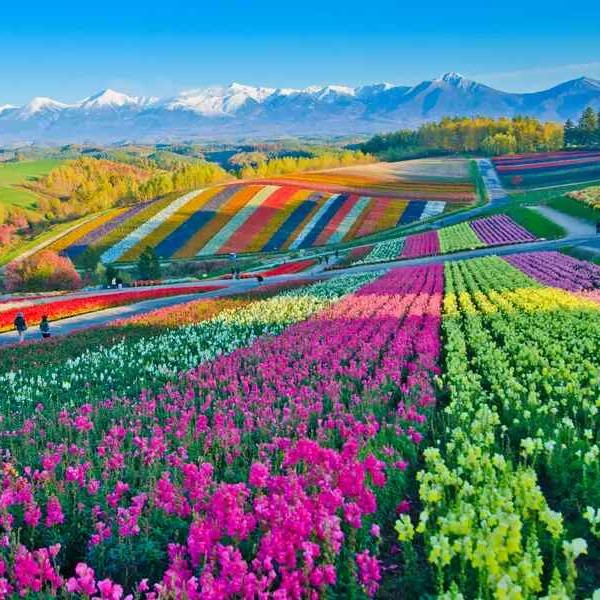
\includegraphics[width=0.4\textwidth]{./sample_inputs/input_image.jpg}
    \caption{Sample Input Image}
  \end{figure*}

  \item \textnormal{Using the image from no. 2, convert the image into grayscale
  and display the image.}

  \begin{figure*}[htb!]
    \centering
    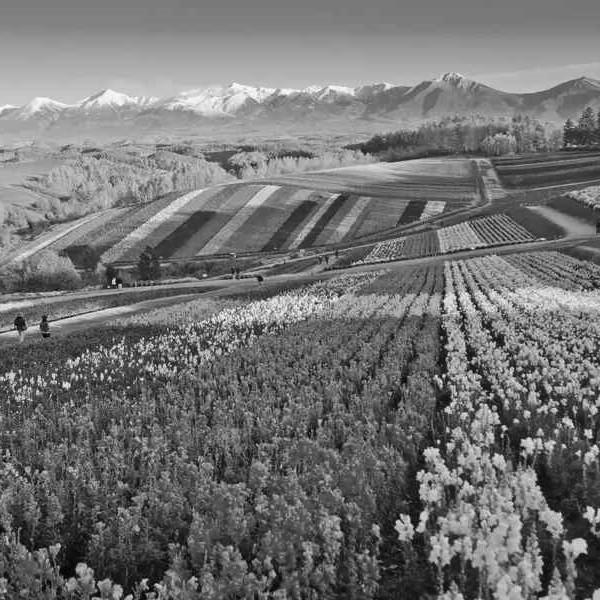
\includegraphics[width=0.4\textwidth]{./sample_outputs/e1_gray_image.jpg}
    \caption{Sample Grayscale Image}
  \end{figure*}

  \item \textnormal{Using the image from no. 3, process the image to `2-bit` and
  display the image.}

  \begin{figure*}[htb!]
    \centering
    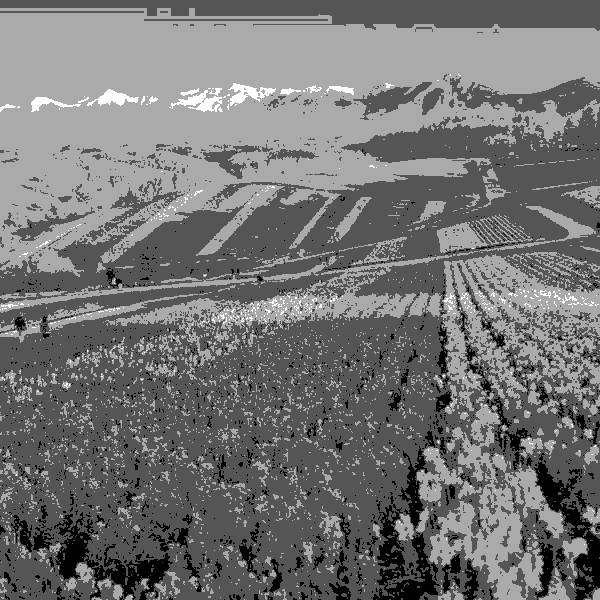
\includegraphics[width=0.4\textwidth]{./sample_outputs/e1_output.png}
    \caption{Sample Output Image (e1\_output.png)}
  \end{figure*}
  
  \item \textnormal{Using the image from no. 4, save the output image in PNG
  format with the name `e1\_output.png` and display the image.}
\end{enumerate}

\subsection*{Exercise 2}

\begin{enumerate}
  \item \textnormal{Write a Python program to read an image from a file using
  OpenCV and display it using Matplotlib.}
  
  \begin{figure*}[htb!]
    \centering
    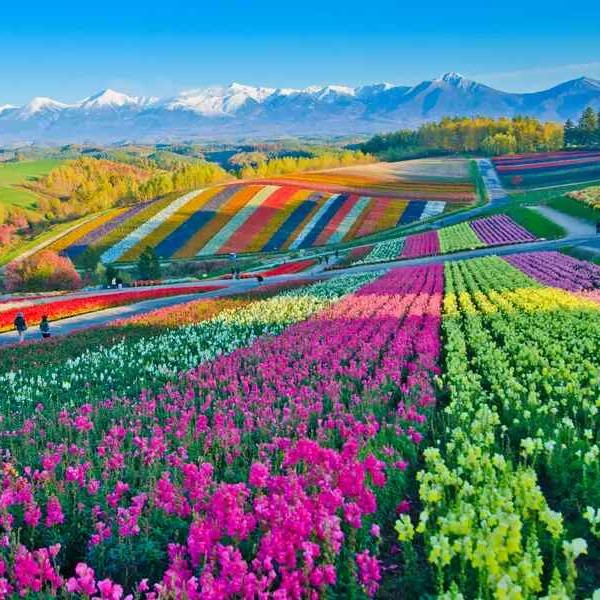
\includegraphics[width=0.4\textwidth]{./sample_inputs/input_image.jpg}
    \caption{Sample Input Image}
  \end{figure*}

  \item \textnormal{Using the image from no. 1, convert the image from BGR to
  RGB color space then display it using Matplotlib.}
  \item \textnormal{Using the image from no. 2, convert the image from RGB to
  HSV color space.}
  \item \textnormal{Using the image from no. 3, change the `red` color in the
  image to `orange` using the HSV color space then display the output image
  using Matplotlib.}

  \begin{figure*}[htb!]
    \centering
    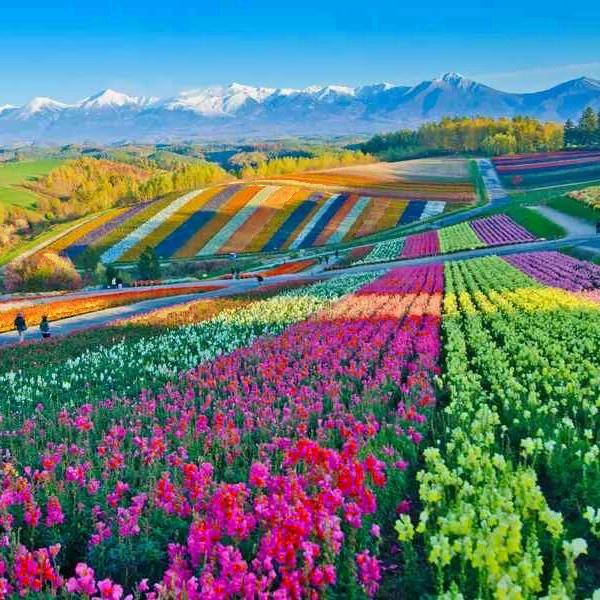
\includegraphics[width=0.4\textwidth]{./sample_outputs/e2_output_ro.jpg}
    \caption{Sample Output Image with Red to Orange Color Change (e2\_output\_ro.jpg)}
  \end{figure*}

  \item \textnormal{Using the image from no. 4, change the `green` color in the
  image to `yellow` using the HSV color space then display the output image
  using Matplotlib.}

  \begin{figure*}[htb!]
    \centering
    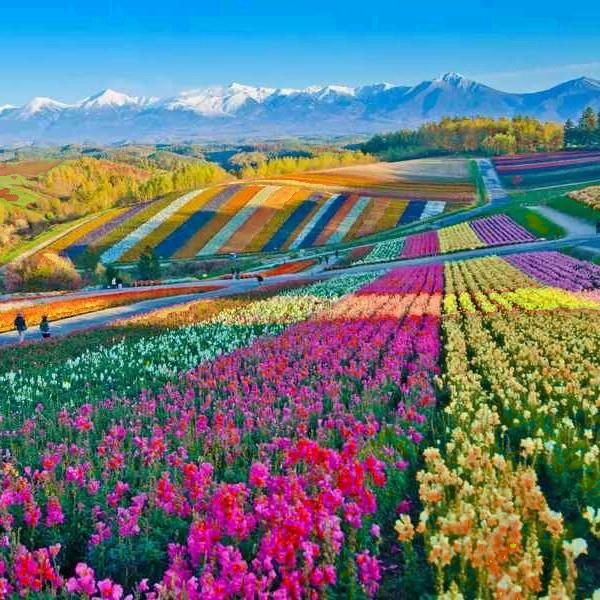
\includegraphics[width=0.4\textwidth]{./sample_outputs/e2_output_gy.jpg}
    \caption{Sample Output Image with Green to Yellow Color Change (e2\_output\_gy.jpg)}
  \end{figure*}

  \item \textnormal{Using the image from no. 5, change the `blue` color in the
  image to `purple` using the HSV color space then display the output image
  using Matplotlib.}

  \begin{figure*}[htb!]
    \centering
    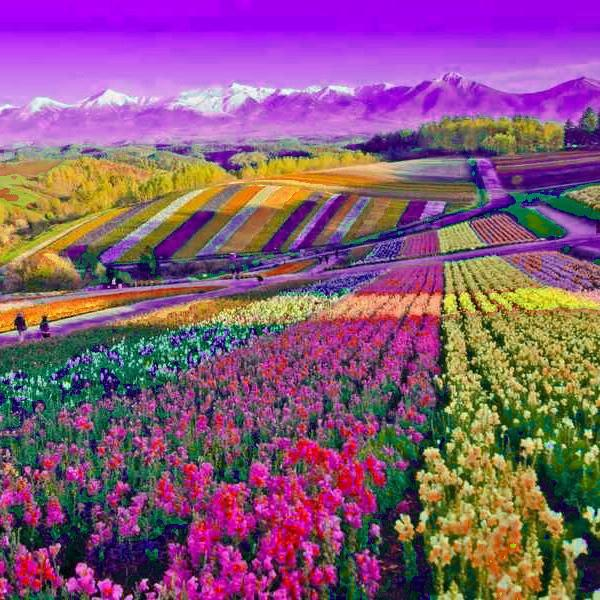
\includegraphics[width=0.4\textwidth]{./sample_outputs/e2_output_bp.jpg}
    \caption{Sample Output Image with Blue to Purple Color Change (e2\_output\_bp.jpg)}
  \end{figure*}

  \item \textnormal{Save the output images from no. 4, 5, and 6 with the
  following names:}
  \begin{enumerate}
    \item \textnormal{`e2\_output\_ro.jpg`}
    \item \textnormal{`e2\_output\_gy.jpg`}
    \item \textnormal{`e2\_output\_bp.jpg`}
  \end{enumerate}
\end{enumerate}

\section*{Submission of Coding Exercises}

Instructions:
\begin{enumerate}
  \item Go to the Google Drive folder provided by the instructor: \\
  \begin{quote}
    \textbf{BSCS 3-1:} \\ \url{\GoogleDriveURLBSCSThreeOne} \\ \\
    \textbf{BSCS 3-2:} \\ \url{\GoogleDriveURLBSCSThreeTwo}
  \end{quote}
  \item Inside the folder, create another folder for your group
  with the following format:
    \begin{quote}
      \textbf{\FolderFormat} \\
      Example: \textbf{\FolderFormatExample}
    \end{quote}
  \item Inside the sub-folder, create another folder with the name:
    \begin{quote}
        \textbf{Chapter \ChapterNumber - Coding Exercise \CodingNumber - \CodingTitle}
    \end{quote}
  \item Inside the folder, upload the file of your submission.
    \begin{quote}
        Fill in the template provided in the following link and upload
        it inside the folder: \\
        \url{\SubmissionTemplateURL}
    \end{quote}
  \item The activity must be submitted \textbf{\SubmissionDeadlineText}.
  \item Late submissions will not be accepted.
\end{enumerate}

\end{document}